
\section{Additive models}
A linear model has the form $\alpha + f_1(X_1) + f_2(X_2) + f_3(X_3) + \cdots$, where $X$ are the predictors.

\subsection{Tree based methods}
Tree-based methods partition the feature space into a set of rectangles, and then fit a simple model (like a constant) in each one.

We restrict attention to recursive binary partitions. We first split the space into two regions, and model the response by the mean of $Y$ in each region. We choose the variable and split-point to achieve the best fit. Then one or both of these regions are split into two more regions, and this process is continued, until some stopping rule is applied.

For example we first split at $X_1 = t_1$. Then the region $X_1 \le t_1$ is split at $X_2 =t_2$ and the region $X_1 >t_1$ is split at $X_1 =t_3$ and so on. To each sub-region we assign a constant as output:
\begin{equation}
\hat{f}(X) = \sum_{m=1}^M c_m I\{(\x \in \CMcal{R}_m\}
\end{equation}
An advantage of this representation is its interpretability. When more than 2 inputs are involved, it is difficult to represent the partition of the input space. 
\begin{figure}
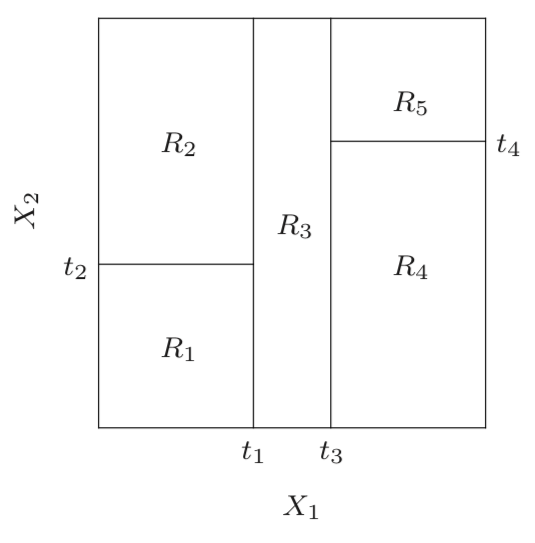
\includegraphics[scale=0.4]{img/tree1}
\caption{2D-input space binary tree partition.}
\label{tree1}
\end{figure}
\begin{figure}
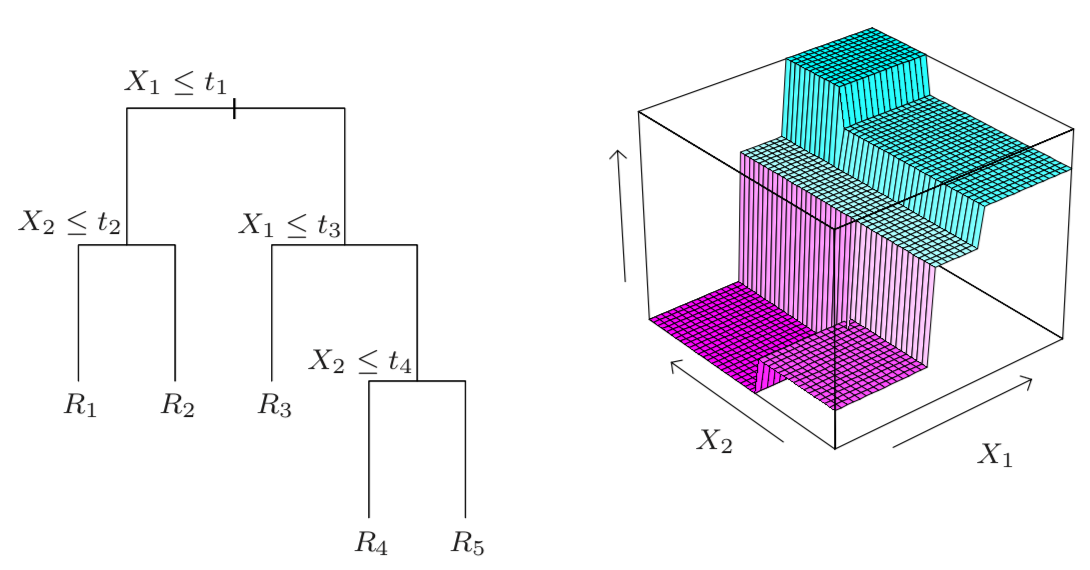
\includegraphics[scale=0.39]{img/tree2}
\caption{Another representation of the binary tree on the left. On the right the 3D resulting shape of the function.}
\label{tree2}
\end{figure}
\subsubsection{Regression Trees}
The algorithm needs to decide automatically the splitting variables and points. We can start defining the values of the constant of each region:
\begin{equation}
\hat{c}_m = ave(y_i|x_i \in \CMcal{R}_m)
\end{equation}
Now finding the best binary partition in terms of minimum sum of squares is generally computationally infeasible. Hence we proceed with a greedy algorithm. Consider a splitting variable $j$ and split point $s$ and define the pair of half-planes:
\begin{equation}
R_1(j,s) = \{X|X_j \le s \}. \quad R_2(j,s) = \{X|X_j > s \}
\end{equation}
Then we seek the splitting variable $j$ and split point $s$ that solve:
\begin{equation}
\begin{aligned}
&\min_{j,s}\left[ \min_{c_1} \sum_{x_i \in \CMcal{R}_1(j,s)}  (y_i-c_1)^2 + \min_{c_2} \sum_{x_i \in \CMcal{R}_2(j,s)}  (y_i-c_2)^2\right]\\
&\hat{c}_1 = ave (y_i|x_i \in R_1(j,s)) \\
&\hat{c}_2 = ave (y_i|x_i \in R_2(j,s)) 
\end{aligned}
\end{equation}
For each splitting variable, the determination of the split point s can be done very quickly and hence by scanning through all of the inputs, determination of the best pair $(j, s)$ is feasible. Having found the best split, we partition the data into the two resulting regions and repeat the splitting process on each of the two regions. Then this process is repeated on all of the resulting regions.


Tree size is a tuning parameter governing the model's complexity, and the optimal tree size should be adaptively chosen from the data. One approach would be to split tree nodes only if the decrease in sum-of-squares due to the split exceeds some threshold. This strategy is too short-sighted, however, since a seemingly worthless split might lead to a very good split below it.
The preferred strategy is to grow a large tree $T_0$, stopping the splitting process only when some minimum node size (say 5) is reached. Then this large tree is pruned using \textbf{cost-complexity pruning}.

The \textbf{cost-complexity pruning} is the following. We define a subtree $T$ of $T_0$. obtained by collapsing any number of its internal nodes. We index the terminal nodes by $m$. let $|T|$ denote the number of terminal nodes in $T$ and 
\begin{equation}
\begin{aligned}
N_m &= \#\{x_i \in \CMcal{R}_m\}\\
\hat{c}_m &= \frac{1}{N_m} \sum_{x_i \ in \CMcal{R}_m} y_i\\
Q_m(T) &= \frac{1}{N_m} \sum_{x_i \in R_m}(y_i - \hat{c}_m)^2
\end{aligned}
\end{equation} 
We define the cost complexity criterion:
\begin{equation}
C_\alpha (T) = \sum_{m=1}^{|T|} N_m Q_m(T) + \alpha |T|
\end{equation}
The idea is to find for each $\alpha$ the subtree $T_\alpha$ of $T_0$ to minimize such a function.
For each $\alpha$ there is a unique smallest subtree $T_\alpha$ that minimizes $C_\alpha(T)$. To find $T_\alpha$ we use the \textbf{weakest link pruning}: we collapse the internal node that produces the smallest per-node increase and we continue umtil we produce the single-node (root) tree. So we have a sequence of subtrees that must contain $T_\alpha$. We choose $\alpha$ to minimize the cross-validated sum of squares, obtaining the tree $T_\alpha$.

\subsection{Classification trees}
The procedure is very similar. In a node $m$ representing the region $R_m$ with $N_m$ observations, let 
\begin{equation}
\hat{p}_{mk} = \frac{1}{N_m}\sum_{\x_i\in R_m} I(y_i=k)
\end{equation}
We classify the observations in node $m$ to class
\begin{equation}
k(m) =argmax_k \hat{p}_{mk},
\end{equation}
the majority class in node $m$. Different measures $Q_m(T)$ of node impurity exist
\begin{equation}
\begin{aligned}
&\textbf{Misclassification error} \quad \frac{1}{N_m} \sum_{i\in \CMcal{R}_m} I(y_i \ne k(m))=1-\hat{p}_{km}\\
&\textbf{Gini index} \quad\quad \sum_{k\ne k'} \hat{p}_{mk}\hat{p}_{mk'} = \sum_{k=1}^K \hat{p}_{mk}(1- \hat{p}_{mk})\\
&\textbf{Cross-entropy or deviance} \quad -\sum_{k=1}^K \hat{p}_{mk}\log \hat{p}_{mk}
\end{aligned}
\end{equation}

These trees are referred as CART (classification and regression trees).
\subsubsection{Linear Combination splits}
Rather than using splits of the type $X_j\le s$ we can use splits of the type $\sum a_j X_j \le s$. The weights $a_j$ and split point $s$ are optimized to minimize the relevant criterion  such as the Gini index.

\subsubsection{Limitations of trees}
One major problem of trees is \textbf{the instability (i.e., high variance)}. A small change in the data can result in a very different series of splits, making interpretation somewhat precarious. The major reason is the hierarchical nature of the process: the effect of an error in the top split is propagated down to all the next splits. The problem can be attenuated but not completely solved.

Another problem of trees is the \textbf{lack of smoothness}. This is not a problem in classification but it is in regression.

Also they are not good at capturing additive structures, such as $Y = c_1 (X_1 < t_1) + c_1 (X_1 < t_1)+\epsilon$ where the noise is $0$ mean. Then a binary tree might make its first split on $X_1$ near $t_1$. At the next level down it would have to split both nodes $X_2$ at $t_2$ in order to capture the additive structure. This is achieved with sufficient data, but it it is a fragile mechanism and can fail in case of many additive effects.
\subsection{Patient rule induction method (PRIM)}
Also PRIM finds boxes in the feature space, but it seeks boxes in which the response average is high. Hence it looks for maxima in the target function, an exercise known as bump hunting. The main box construction method in PRIM works starting with a box containing all of the data. The box is compressed along one face by a small amount, and peeling off a constant portion of data denoted by $\alpha$. Typically $\alpha$ is $0.05$ and $0.1$ of the remaining points at each stage. The face chosen for compression is the one resulting in the largest box mean, after the compression is performed. Then the process is repeated, stopping when the current box contains some minimum number of data points.

After the top-down sequence is computed, PRIM reverses the process, expanding along any edge, if such an expansion increases the box mean. This is called pasting. The result of these steps is a sequence of boxes, with different numbers of observation in each box. Cross-validation, combined with the judgement of the data analyst, is used to choose the optimal box size. Denote by $B_1$ the points in this first box. These points are now removed from the training set and we repeat the two processes (top-down peeling and bottom-up pasting) several times, obtaining for each iteration a new box $B_i$. Each box is defined by a set of rules involving a subset of predictors such as:
\begin{equation}
(a_1 \le X_1 \le b_1) \quad\quad (b_1 \le X_3 \le b_2)
\end{equation}
PRIM can handle a categorical predictor by considering all partitions of the predictor, as in CART. Missing values are also handled in a manner similar to CART. PRIM is designed for regression

\begin{algorithm}[!ht]
Start with all of the training data, and a maximal box containing all of the data;\\

Consider shrinking the box by compressing one face, so as to peel off the proportion $\alpha$ of observations having either the highest values of a predictor $X_j$ or the lowest. Choose the peeling that produces the highest response mean in the remaining box;\\

Repeat step 2 until some minimal number of observations (say 10) remain in the box;\\

Expand the box along any face, as long as the resulting box mean increases;\\

Steps 1-4 give a sequence of boxes, with different numbers of observations in each box. Use cross-validation to choose a member of the sequence. Call the box $B_1$.\\

Remove the data in the box $B_1$ from the dataset and repeat steps 2-5 to obtain a second box. and continue to get as many boxes as desired.
\end{algorithm}

\begin{figure}
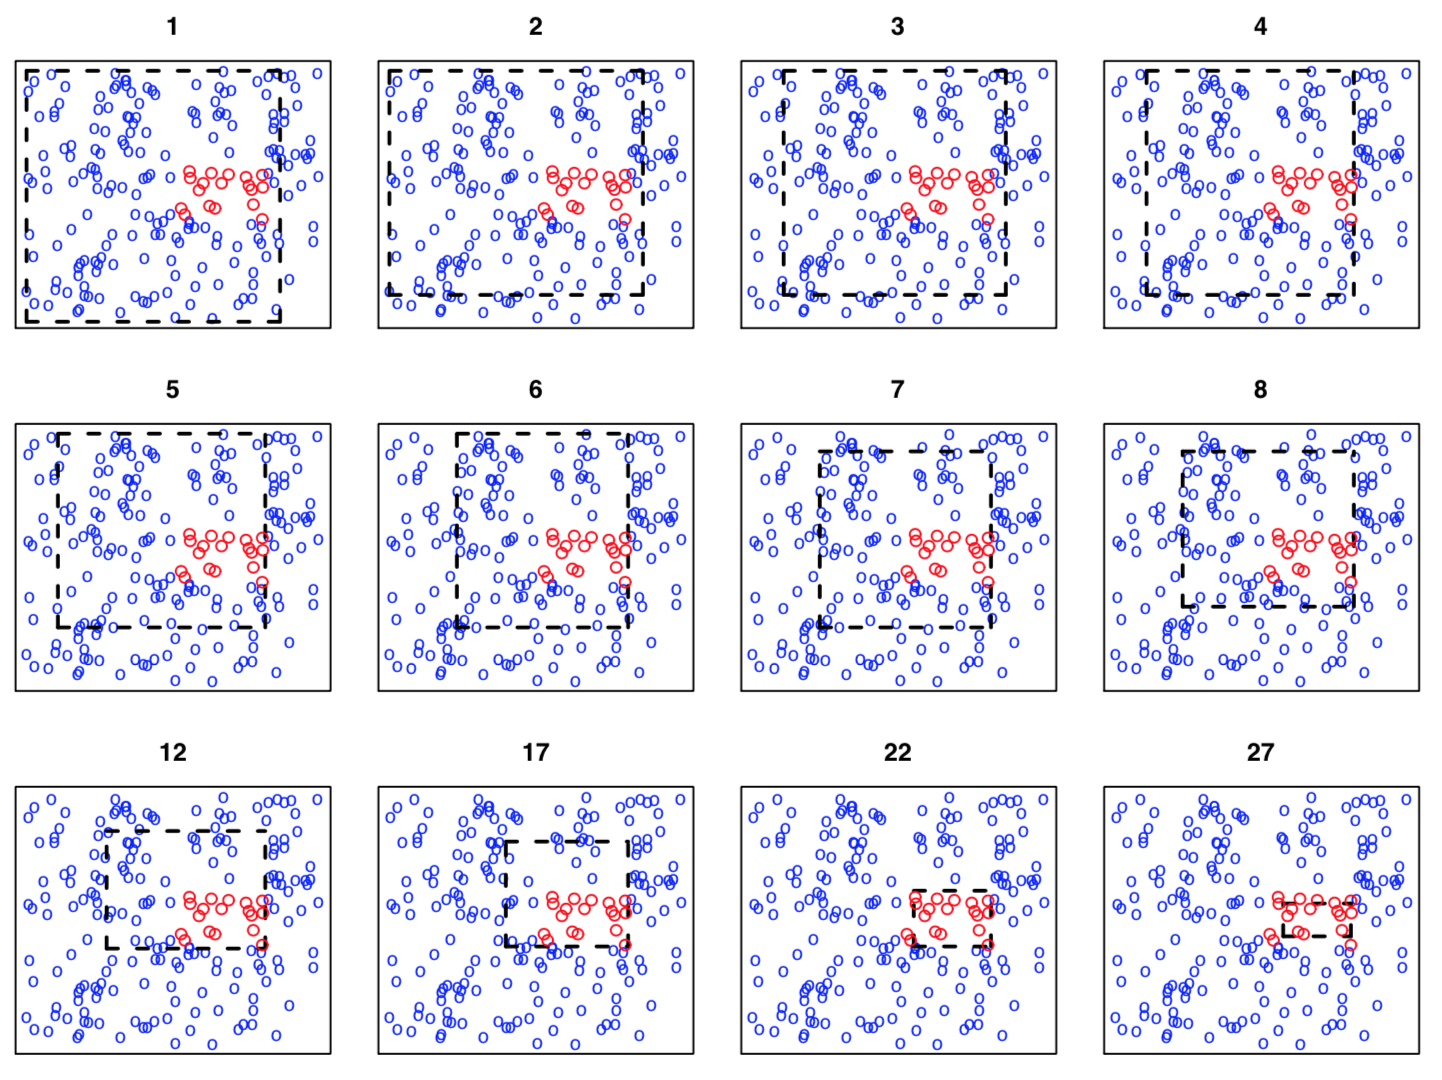
\includegraphics[scale=0.4]{img/PRIM}
\caption{Steps in PRIM.}

\end{figure}
PRIM is designed for binary regression. There is no simple way to deal with $k>2$ classes simultaneously: it is possible to run PRIM separately for each class versus a baseline class.In any case, the ability of PRIM to be more patient should help the top-down greedy algorithm find a better solution.

\subsection{Multivariate Adaptive Regression Splines (MARS)}
It is a procedure well-suited for high-dimensional problems. MARS uses expansions in piecewise linear basis functions of the form $(x-t)_+$ and $(t-x)_+$.

Each function is piecewise linear, with a knot at the value $t_1$. We call the two functions a \textbf{reflected pair}. The idea is to form reflected pairs for each input $X_j$ with knots at each observed value $x_{ij}$ of that input. If all of the input values are distinct, there are $2Np$ basis functions altogether.
The model-building strategy is like a forward stepwise linear regression, but instead of using the original inputs, we are allowed to use functions from the set $\CMcal{C}$ and their products:
\begin{equation}
\CMcal{C} = \{(X_j-t)_+, (t-X_j)_+\}_{t \in \{x_{1j},\cdots, x_{Nj}\}, j=1,\cdots,p}
\end{equation}
Thus the model has the form:
\begin{equation}
f(X) = \beta_0 + \sum_{m=1}^M \beta_m h_m(X)
\end{equation}
where each $h_m(X)$ is a function in $\CMcal{C}$ or a product of two or more such functions. Given the choice for $h_m(X)$, the coefficients are estimated with the residual sum of squares. We start with only a constant $h_0(X)=1$ and all the functions are candidate functions. At each step we consider as a new basis function pair all products of a function $h_m$ in the model set $\CMcal{M}$ with one of the reflected pairs in $\CMcal{C}$. We add to the model $\CMcal{M}$ the term of the form:
\begin{equation}
\hat{\beta}_{M+1}h_\ell(X) (X_j-t)_+ + \hat{\beta}_{M+2}h_\ell(X) (t-X_j)_+, h_\ell \in \CMcal{M}
\end{equation}
that produces the largest decrease in training error. For example, at the first stage we consider adding to the model a function of the form: $\hat{\beta}_1 (X_2-x_{72})_+ + \hat{\beta}_2(x_{72}-X_2)_+$. Then this pair of basis functions is added to the set $\CMcal{M}$ and at the next stage we consider including a pair of products in the form:
\begin{equation}
h_m(X) (X_j-t)_+ \quad\quad \text{and}\quad\quad h_m(X) (t-X_j)_+, t \in \{x{ij}\}
\end{equation}
where for $h_m$ we have the choices:
\begin{equation}
\begin{aligned}
&h_0(X) = 1\\
&h_1(X) = (X_2 - x_{72})_+,  \quad\textit{or}\\
&h_2(X) = (x_{72} - X_2)_+
\end{aligned}
\end{equation}
At the end of this process we have a large model. This model typically overfits the data, and so a backward deletion procedure is applied. The term whose removal causes the smallest increase in residual squared error is deleted from the model at each stage, producing an estimated best model $\hat{f}_\lambda$ of each size (number of terms) $\lambda$. One could use cross-validation to estimate the optimal value of $\lambda$, but for computational savings the MARS procedure instead uses generalized cross-validation:
\begin{equation}
GCV(\lambda) = \frac{\sum_{i=1}^N (y_i - \hat{f}_\lambda(x_i))^2}{(1-\frac{M(\lambda)}{N})^2}
\end{equation}
The value $M(\lambda)$ is the effective number of parameters in the model: this accounts both for the number of terms in the models, plus the number of parameters used in selecting the optimal positions of the knots.

Some mathematical and simulation results suggest that one should pay a price of three parameters for selecting a knot in a piecewise linear regression.
Thus if there are r linearly independent basis functions in the model, and $K$ knots were selected in the forward process, the formula is $M(\lambda) = r+cK$, where $c = 3$.

The MARS method and algorithm can be extended to handle classification problems. Several strategies have been suggested. For two classes, one can code the output as 0/1 and treat the problem as a regression; we did this for the spam example. For more than two classes, one can use the indicator response approach. One codes the $K$ response classes via 0/1 indicator variables, and then performs a multi-response MARS regression. There are, however, potential masking problems with this approach.

\subsection{Hierarchical Mixture of Experts}
This can be viewed as a variant of tree-based methods. The main difference is that the tree splits are not hard decisions but rather soft probabilistic ones. At each node an observation goes left or right with probabilities depending on its input values. In an HME, a linear (or logistic regression) model is fit in each terminal node, instead of a constant as in CART (the split can be multiway, not only binary).

The terminal nodes are called \textbf{experts}, and the non-terminal nodes are called \textbf{gating networks}. The idea is that each expert provides an opinion (prediction) about the response, and these are combined together by the gating networks. The model is formally a mixture model, and the two-level model in the figure can be extend to multiple levels, hence the name hierarchical mixtures of experts.

\begin{figure}
\centering
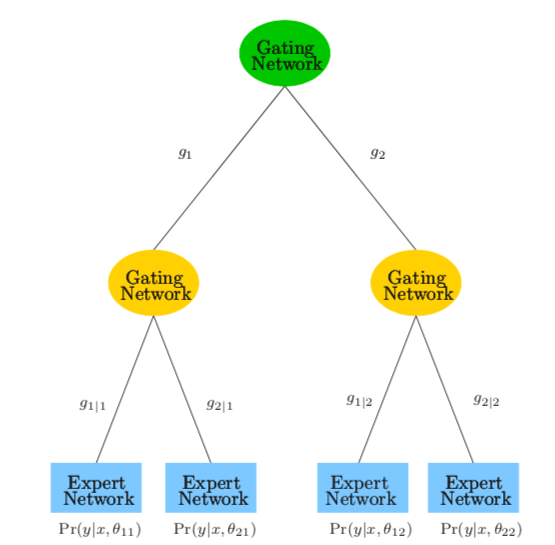
\includegraphics[scale=0.5]{img/HME}
\caption{A two-level HME model.}
\end{figure}
\subsubsection{How HME works}
Consider the data $(x_i, y_i), \quad i=1,\cdots, N$ either for regression or classification problem. The \textbf{top-gating} network has the output:
\begin{equation}
g_j(\x, \gamma_j) = \frac{e^{\gamma_j^T\x}}{\sum_{k=1}^Ke^{\gamma_k^T\x}}, \quad\quad j=1,\cdots, K
\end{equation}
where $\gamma_j$ is a vector of unknown parameters. Each $g_j$ is the probability of assigning an observation with feature vector $\x$ to the $j-th$ branch (soft $K$-way split). At second level the \textbf{gating networks} have similar form:
\begin{equation}
g_{\ell|j}(\x, \gamma_{j|\ell}) = \frac{e^{\gamma_{j|\ell}^T\x}}{\sum_{k=1}^Ke^{\gamma_{j|k}^T\x}}, \quad\quad \ell=1,
\end{equation}
This is the probability of assignment to the $l-th$ branch, given assignment to the $j-th$ branch at the level above. At each expert (terminal node), we have a model for the response variable of the form:
\begin{equation}
Y \sim Pr(y|\x, \theta_{j\ell}
\end{equation}
which is different according to the type of problem. For \textbf{regression} the Gaussian linear model is used with $\theta_{j\ell} = (\beta_{j\ell},\sigma^2_{jl}$:
\begin{equation}
Y = \beta_{j\ell}^Tx + epsilon, \quad\quad \CMcal{N} \sim(0,\sigma^2_{jl}). 
\end{equation}

For \textbf{classification} the linear logistic regression is used:
\begin{equation}
Pr(Y=1|\x, \theta_{j\ell} = \frac{1}{1+e^{-\theta_{j\ell}^T\x}}
\end{equation}
Denoting with $\Phi = \{\gamma_j,\gamma_{j\ell}, \theta_{j\ell}\}$ the collections of all parameters, the total probability that $Y=y$ is:
\begin{equation}
Pr(y|\x, \Phi) = \sum_{k=1}^K g_j(x, \gamma_j)\sum_{\ell=1}^K g_{\ell|j}(\x, \gamma_{j\ell})Pr(y|\x,\theta_{j\ell})
\end{equation}
To estimate the parameters we maximize the log-likelihood of the data over $\Phi$. The most convenient method is the EM algorithm.

\subsection{Missing data}
The usual approach is to fill-in missing values. Roughly speaking, data are missing at random if the mechanism resulting in its omission is independent of its (unobserved) value. A more precise definition is given in Little and Rubin (2002). Suppose $y$ is the response vector and $X$ is the $N \times p$ matrix of inputs (some of which are missing). Denote by $X_{obs}$ the observed entries in $X$ and let $\mathbf{Z} = (y, X)$, $\mathbf{Z}_{obs} = (\y, \X_{obs})$. Finally, if $\mathbf{R}$ is an indicator matrix with $ij-th$entry 1 if $x_{ij}$ is missing and zero otherwise, then the data is said to be missing at random (MAR) if the distribution of $\mathbf{R}$ depends on the data $\mathbf{Z}$ only through $Z_{obs}$:
\begin{equation}
Pr(\mathbf{R}|\mathbf{Z},\theta) = Pr (\mathbf{R}|\mathbf{Z}_{obs},\theta)
\end{equation}
Data are said to be \textbf{missing completely at random (MCAR)} if the distribution$\mathbf{R}$ does not depend on the observed or missing data:
\begin{equation}
Pr(\mathbf{R}|\mathbf{Z},\theta) = Pr (\mathbf{R}|\theta)
\end{equation}
For example, if a patient’s measurement was not taken because the doctor felt he was too sick, that observation would not be MAR or MCAR.

Assuming the features are missing completely at random, there are a number of ways of proceeding:

\begin{enumerate}
\item \label{Missingi}Discard observations with any missing values.
\item \label{Missingii}Rely on the learning algorithm to deal with missing values in its training phase.
\item \label{Missingiii}Impute all missing values before training.
\end{enumerate}

Approach \autoref{Missingi} can be used if the relative amount of missing data is small, but otherwise should be avoided. Regarding \autoref{Missingii}, CART is one learning algorithm that deals effectively with missing values, through surrogate splits. MARS and PRIM use similar approaches. In generalized additive modeling, all observations missing for a given input feature are omitted when the partial residuals are smoothed against that feature in the backfitting algorithm, and their fitted values are set to zero. Since the fitted curves have mean zero (when the model includes an intercept), this amounts to assigning the average fitted value to the missing observations.
For most learning methods, the imputation approach \autoref{Missingiii} is necessary. The simplest tactic is to impute the missing value with the mean or median of the non-missing values for that feature.

If the features have at least some moderate degree of dependence, one can do better by estimating a predictive model for each feature given the other features and then imputing each missing value by its prediction from the model, distinctly from the method used to predict $y$ from $\x$.